%%$Id: thesis-e.tex,v 1.4 2003/01/20 06:05:12 gondow Exp $
\documentclass[12pt]{report}
\usepackage{jaist-e-master}
\usepackage{llncsdoc}
\usepackage{verbatim}
\usepackage[numbers]{natbib}
\usepackage{graphics}
\usepackage{graphicx}
\usepackage{caption}
\usepackage{subcaption}

% *** MISC UTILITY PACKAGES ***
%
\usepackage{siunitx}
\usepackage{amsthm}
\newtheorem{definition}{Definition}[section]
\newtheorem{theorem}{Theorem}[section]
%\newtheorem{proof}{Proof}
\newtheorem{example}{Example}[section]
\newtheorem{lemma}{Lemma}[section]
\usepackage{amssymb}
\setcounter{tocdepth}{3}
\usepackage{tikz} 
\usepackage{graphicx}
\graphicspath{ {Figs/} }

\usepackage{amsmath}
\usepackage{multirow}
\usepackage{slashbox}
\usepackage{amsfonts}

\usepackage{algpseudocode}
\usepackage{algorithm}
\usepackage{epstopdf}
\usepackage{array}
\usepackage{enumerate}

\usepackage{epstopdf}

\usepackage{url}
%\urldef{\mailsa}\path|{khanhtv, mizuhito}@jaist.ac.jp|    

%ieee requirements
%\usepackage[utf8]{inputenc}
%\usepackage[T1]{fontenc}
%\usepackage{microtype} 
%\usepackage{balance}

%user definitions
\newcommand{\Nat}{{\mathbb N}}
\newcommand{\Real}{{\mathbb R}}
\newcommand{\Rat}{{\mathbb Q}}
\newcommand{\suppress}[1]{} % Comment out text.
\newcommand{\mizuhito}[1]{\{{\bf Mizuhito:~\sf #1}\}} % Highlight text.
\newcommand{\khanh}[1]{\{{\bf Khanh:~\sf #1}\}} % Highlight text.

\newcommand{\smallHead}[1]{%
    \par\vspace{.35cm}\noindent\textbf{#1}%
    \par\noindent\ignorespaces%
}

\newcommand\TTTT{%
 \textsf{T\kern-0.2em\raisebox{-0.3em}T\kern-0.2emT\kern-0.2em\raisebox{-0.3em}2}%
}

% correct bad hyphenation here
\hyphenation{op-tical net-works semi-conduc-tor}
%
\title{Equality handling and efficiency improvement of SMT for non-linear constraints over reals}%% title 
\author{VU XUAN TUNG}{1310007}                %% author's name
\school{Information Science}                 %% school
\adviser{Professor Mizuhito Ogawa}   %% your adviser
\judge{Professor Mizuhito Ogawa}     %% chief judge
      {Associate Professor Nao Hirokawa}            %% judge 
      {Professor Tachio Terauchi} %% judge
\date{February, 2015}{March, 2015}
   %% submitted date (month, year), graduated date (month, year)

\begin{document}
\maketitle

\begin{abstract}
This thesis presents strategies for efficiency improvement and extensions of an SMT solver {\bf raSAT} for polynomial constraints. 
\begin{comment}
Solving polynomial constraints is raised from many applications of Software Verification such as roundoff/overflow error analysis, automatic termination proving or loop invariant generation. In 1948, Tarski proved the decidability of polynomial constraints over real numbers by proposing a decision method \cite{tarski} which is, however, "totally impractical" \cite{Davenport198829}. Later in \citeyear{Collins:1976:QER:1093390.1093393} \citet{Collins:1976:QER:1093390.1093393} introduced an algorithm called Cylindrical Algebraic Decomposition (CAD) which is complete but its time complexity is doubly-exponential with respect to the number of variables. A number of incomplete methodologies have been also proposed. MiniSmt employs bit-blasting method which is "dedicated to satisfiable instances only" \cite{Zankl:2010:SNR:1939141.1939168}. Virtual Substitution which is implemented in SMT-RAT \cite{smtrat} and Z3 \cite{PBM12} requires polynomials with degree less than $5$. CORD \cite{cordic} linearizes each multiplication as a sequence of linear constraint (with new variables) which makes the size of the problem become large when high degree polynomials present. Another approach is Interval Constraint Propagation (ICP) which use the inequalities/equations to contract the interval of variables by removing the unsatisfiable intervals. ICP uses floating point arithmetic so it does not suffers from high degree of polynomial, bt the number of boxes (combination of intervals of variables) may grow exponentially. As a result, ICP-based solvers need to have strategies to overcome this drawback.
\end{comment}

{\bf raSAT} which initially focuses on polynomial inequalities over real numbers follows ICP methodology and adds testing to boost satisfiability detection \cite{VanKhanh201227}. In this work, in order to deal with exponential exploration of boxes, several heuristic measures, called {\em SAT likelyhood}, {\em sensitivity}, and the number of 
unsolved atomic polynomial constraints, are proposed. Extensions for handling equations and handling constraints over integer number are also presented.
\end{abstract}

\chapter*{\centering Acknowledgements}
\noindent I would like to express my sincere gratitude to my supervisor, Professor Mizuhito Ogawa for the continuous support of not only my thesis but also my life. He instructed me how to critically think about and evaluate research.\\\\
My sincere thanks also goes to Associate Professor Nao Hirokawa for his detailed and constructive comments and also for his important support through this work. I learned a lot from him how to write scientific documents. \\\\
I owe my loving thanks to my parents, my older brother, my older sister and my girl friend. Without their encouragement and understanding it would have been impossible for me to finish this work.

\tableofcontents

%\listoffigures
 
%\listoftables

\chapter{Introduction}
\section{Polynomial constraint solving}
{\em Polynomial constraint solving over real numbers} is a task of computing an assignment of real values to variables
that satisfies given polynomial inequalities/equations. If such an assignment exists, the constraint is said to be satisfiable (SAT) and the assignment is called SAT instance; otherwise we mention it as unsatisfiable (UNSAT). 
\begin{example} \label{examp:unsat-example}
$x^2 + y^2 < 1 \wedge xy > 1$ is an example of an UNSAT constraint. While the set of satisfiable points for the first inequality ($x^2 + y^2 < 1$) is the read circle in Figure \ref{fig:unsat-example}, the set for the second one is the green area. Because these two areas do not intersect, the conjunction of two equalities is UNSAT.
\end{example}

\begin{figure}[ht]
%\begin{minipage}[b]{1.0\linewidth}
\centering
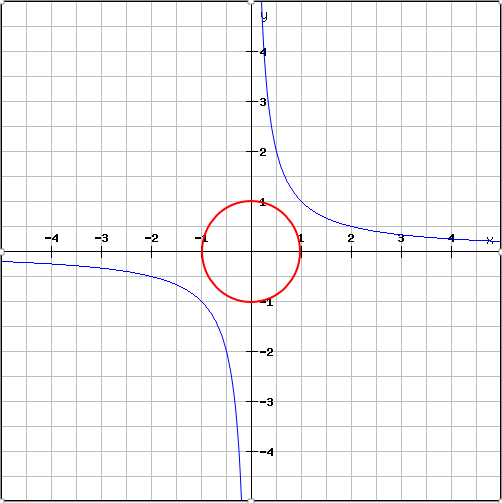
\includegraphics{UNSAT-example.png} 
\caption{Example of UNSAT constraint} 
\label{fig:unsat-example} 
%\end{minipage}
\end{figure} 

\begin{example} \label{examp:sat-example}
Figure~\ref{fig:sat-example} illustrates the satisfiability of the constraint: $x^2 + y^2 < 4 \wedge xy > 1$. Any point in the purple area is a SAT instance of the constraint, e.g. $(1.5, 1)$.
\end{example}

\begin{figure}[ht]
%\begin{minipage}[b]{1.0\linewidth}
\centering
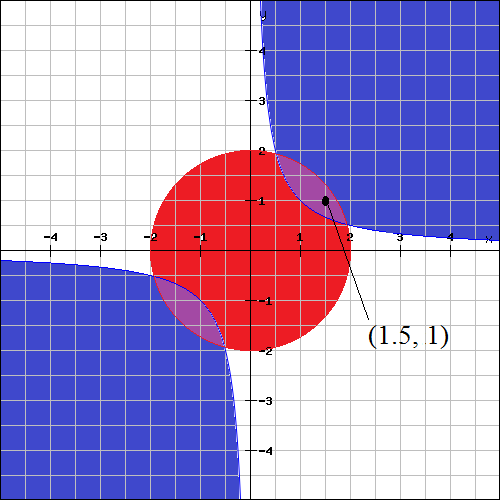
\includegraphics{SAT-example.png} 
\caption{Example of SAT constraint} 
\label{fig:sat-example} 
%\end{minipage}
\end{figure} 

%For instance, $\exists x y. -y^2 + (x^2 - 1) y - 1 > 0 \wedge -x^2 - y^2 + 4 > 0$ is 
%such an example. This is an easy formula, but proving its satisfiability and 
%showing a satisfiable instance (e.g., $x = 1.8$, $y=0.9$) are not so easy.  
%its satisfiability and a satisfiable instance 
%(e.g., $x = 1.8$, $y=0.9$) are not so easy.  		
%
Solving polynomial constraints has many application in Software Verification, such as 
\begin{itemize}
\item {\bf Locating roundoff and overflow errors}, 
which is our motivation~\cite{Ngoc:2009:ORE:1685167.1685421,Ngoc:2010:CRE:1858996.1859056}
%DSP decorders in practice are defined by reference algorithms in C using floating point arithmetic. 
%In embedded systems, often it is replaced with fixed point arithmetic, 
%which may cause visible noises. 
%and locating such roundoff error source is not easy. 
%For instance, consider DSP decoder like mpeg4. Usually, the decoder definition is given by a reference 
%algorithm in C, which uses floating point number. 
%In an embedded system, it is tempting to replace floating 
%point into fixed point numbers. However, naive replacement would cause 

\item {\bf Automatic termination proving}, 
which reduces termination detection to finding a suitable ordering~\cite{Lucas:2008:CCS:1361735.1361760}, 
e.g., \TTTT~\footnote{\url{http://cl-informatik.uibk.ac.at/software/ttt2/}}, 
AProVE~\footnote{\url{http://aprove.informatik.rwth-aachen.de}}. 
%as a solution of polynomial constraints. 

\item {\bf Loop invariant generation}. 
Farkas's lemma is a popular approach in linear loop invariant generation~\cite{Colon}, 
and is reduced to degree $2$ polynomials. 
%matrix multiplications. 
%degree $2$ polynomial constraints. 
%Farkas's lemma uses products of matrices, and it requires solving polynomial constraints of degree 2.
Non-linear loop invariant~\cite{Sankaranarayanan:2004:NLI:982962.964028} requires more complex polynomials.

\item {\bf Hybrid system}. SMT for QF\_NRA are often used as backend engines~\cite{Sankaranarayanan04constructinginvariants}. 

\item {\bf Mechanical contrnol design}. 
PID control is simple but widely used, and designing parameters is 
reduced to polynomial constraints~\cite{control}. 
%Fujitsu used polynomial constraints solving to design PID control of HDD head movement
\end{itemize}	

\section{Existing approaches}
Although solving polynomial constraints on real numbers is decidable~\cite{tarski}, current methodologies have their own pros and cos. They can be classified into the following categories: 
\begin{enumerate}
\item \textbf{Quantifier elimination by cylindrical algebraic decomposition (QE-CAD)}~\cite{qecad} 
is a complete technique, and 
is implemented in Mathematica, Maple/SynRac, Reduce/Redlog, QEPCAD-B, and recently 
in
Z3 4.3 (which is referred as nlsat in~\cite{Jovanovic13}).
Although QE-CAD is precise and detects beyond SAT instances (e.g., SAT regions), 
scalability is still challenging, since its complexity is doubly-exponential with respect to the number of variables. 
%Since QE-CAD is DEXPTIME wrt the number of variables, 

\item \textbf{Virtual substitution } eliminates an existential quantifier by substituting the corresponding quantified variable with a very small value ($-\infty$), and either each root (with respect to that variable) of polynomials appearing in the constraint or each root plus an infinitesimal $\epsilon$. Disjunction of constraints after substitutions is equivalent to the original constraint. Because VS needs the formula for roots of polynomials, its application is restricted to polynomials of degree up to 4. SMT-RAT and  
Z3 \cite{PBM12} applies VS.

\item \textbf{Bit-blasting}. 
In this category of methodology, numerical variables are represented by a sequence of binary variables. The given constraint is converted into another constraint over the boolean variables. SAT solver is then used to find a satisfiable instance of binary variables which can be used to calculate the values of numerical variables.  MiniSmt~\cite{Zankl:2010:SNR:1939141.1939168}, the winner of QF\_NRA in SMT competition 2010, 
applies it for (ir)-rational numbers.
It can show SAT quickly, but due to the bounded bit encoding, 
it cannot conclude UNSAT. In addition, high degree of polynomial results in large SAT formula which is an obstacle of bit-blasting.

\item \textbf{Linearization}. ~
CORD \cite{cordic} uses COrdinate Rotation DIgital Computer (CORDIC) for real numbers to linearizes multiplications into a sequence of linear constraints. Each time one multiplication is linearized, a number of new constraints and new variables are introduced. As a consequence, high degree polynomials in the original constraint lead to large number of linear constraints. 

\item \textbf{Interval Constraint Propagation (ICP)} 
which are used in SMT solver community, e.g., iSAT3~\cite{isat}, 
dReal~\cite{dRealCADE13}, and RSOLVER~\cite{rsolver}. 
ICP combines over-approximation by interval arithmetics and constraint propagation to prune out the set of unsatisfiable points. When pruning does not work, decomposition (branching) on intervals is applied. 
ICP which is capable of solving "multiple thousand arithmetic constraints over some thousands of variables" \cite{isat} is practically often more efficient than algebraic computation.
\end{enumerate}

\section{Proposed Approach and Contributions}
Our aim is an SMT solver for solving polynomial constraint. We first focus on strict inequalities because of the following reasons.
\begin{enumerate}
\item
Satisfiable inequalities allow over-approximation. An over-approximation estimates the range of a polynomial $f$ as $O.range(f)$ that covers all the possible values of $f$, i.e. $range(f) \subseteq O.range(f)$. For an inequality $f>0$, if $O.range(f)$ stays in the positive side, it can be concluded as SAT. On the other hand, over-approximation cannot prove the satisfiability of SAT equations.
\item
Satisfiable inequalities allow under-approximation. An under-approximation computes the range of the polynomial $f$ as  $U.range(f)$ such that $range(f) \supseteq U.range(f)$. If $U.range(f)$ is on the positive side, $f > 0$ can be said to be SAT. Due to the continuity of $f$, finding such an under-approximation for solving $f > 0$ is more feasible than that for $f = 0$.
\begin{itemize}
\item If $f(\bar{x}) > 0$ has a real solution $\bar{x_0}$, there exist rational points near $\bar{x_0}$ which also satisfy the inequality. Solving inequalities over real numbers thus can be reduced to that over rational numbers.
\item The real solution of $f(\bar{x}) = 0$ cannot be approximated to any rational number.
\end{itemize}
\end{enumerate}
For UNSAT constraint (both inequalities and equations) can be solved by over-approximation. Suppose $O.range(f)$ is the result of an over-approximation for a polynomial $f$.
\begin{enumerate}
\item If $O.range(f)$ resides on the negative side, $f > 0$ is UNSAT.
\item If $O.range(f)$ stays on either negative or positive side, $f = 0$ is UNSAT.
\end{enumerate}

Our approach of "iterative approximation refinement" - \textbf{raSAT} loop for solving polynomial constraint was proposed and implemented as an SMT solver named raSAT in \cite{VanKhanh201227}. This work improves the efficiency of the tool and extend it to handle equations. The summary of the proposed method in \cite{VanKhanh201227} is:
\begin{enumerate}
\item Over-approximation is used for both disproving and proving polynomial inequalities. In addition, under-approximation is used for boosting SAT detection. When both of these methods cannot conclude the satisfiability, the input formula is refined so that the result of approximation become more precise. 
\item Interval Arithmetic (IA) and Testing are instantiated as an over-approximation and an under-approximation respectively. While IA defines the computations over the intervals, e.g. $[1, 3] +_{IA} [3, 6] = [2, 9]$, Testing attempts to propose a number of assignments from variables to real numbers and check each assignment against the given constraint to find a SAT instance.
\item In refinement phase, intervals of variables are decomposed into smaller ones. For example, $x \in [0, 10]$ becomes $x \in [0, 4] \vee x \in [4, 10]$.
\item \citet{VanKhanh201227} also proposed a method for detecting satisfiability of equations using the Intermediate Value Theorem.
\end{enumerate}

The contributions of this work are as follows:
\begin{enumerate}
\item Although the method of using IA is robust for large degrees of polynomial, the number of boxes (products of intervals) grows exponentially with respect to the number of variables during refinement (interval decomposition). As a result, strategies for selecting variables to decomposed and boxes to explore play a crucial role in efficiency. We introduce the following strategies:
\begin{itemize}
\item A box with more possiblity to be SAT is selected to explore, which is estimated by 
several heuristic measures, called {\em SAT likelyhood}, 
and the number of unsolved atomic polynomial constraints.
\item A more influential variable is selected for multiple test cases and decomposition. 
This is estimated by {\em sensitivity} which is determined during the computation of IA.
\end{itemize}
\item Two schemes of incremental search are proposed for enhancing solving process: 
\begin{itemize} 
\item {\bf Incremental deepening}. 
raSAT follows the depth-first-search manner. In order to escape local optimums, it starts searching with a threshold that each interval will be decomposed no smaller than it. 
If neither SAT nor UNSAT is detected, a smaller threshold is taken and raSAT restarts. 
\item {\bf Incremental widening}. 
Starting with a small interval, if raSAT detects UNSAT, input intervals are enlarged
and raSAT restarts. For SAT constraint, small (finite) interval allows sensitivity to be computed because Affine Interval \cite{VanKhanh201227} requires finite range of variables. As a consequence, our above strategies will take effects on finding SAT instance. For the UNSAT case, combination of small intervals and incremental deepening helps raSAT quickly determines the threshold in which unsatisfiability may be proved by IA. 
\end{itemize} 
\begin{comment}
SAT-likelihood is introduced to measure the possibility of an inequality to be satisfiable. Sensitivity is proposed to estimate the influence of a variable to the value of a polynomial.
\end{comment}
\item SAT confirmation step by an error-bound guaranteed floating point package {\bf iRRAM}\footnote{% 
\tt http://irram.uni-trier.de}, to avoid soundess bugs caused by roundoff errors.
\item This work also implement the idea of using Intermediate Value Theorem to show the satisfiability of equations which was suggested in \cite{VanKhanh201227}.
\item We also extend raSAT to handle constraint over integer numbers. For this extension, we only generate the integer values for variables in testing phase. In addition, the threshold used for stopping decomposition is set to $1$.
\end{enumerate}
\begin{comment}
\subsection{Inequalities}
Constraints with inequalities can be categorized into four cases:
\begin{enumerate}
\item \textbf{SAT with without touching}
\begin{figure}[ht]
%\begin{minipage}[b]{1.0\linewidth}
\centering
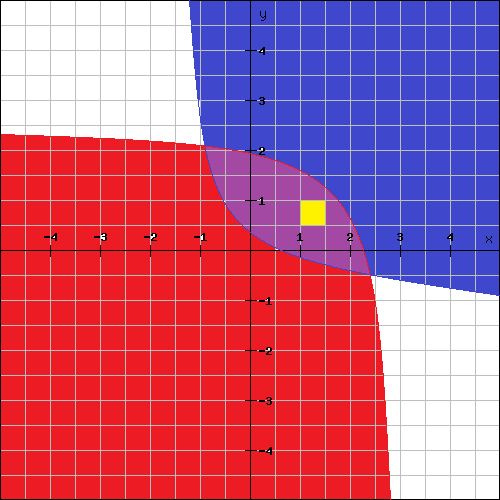
\includegraphics{SAT-withoutTouching.png} 
\caption{SAT without touching dectected by ICP} 
\label{fig:sat-withoutTouching} 
%\end{minipage}
\end{figure} 

\item \textbf{SAT/UNSAT with touching/convergence}
\begin{figure}[ht]
%\begin{minipage}[b]{1.0\linewidth}
\centering
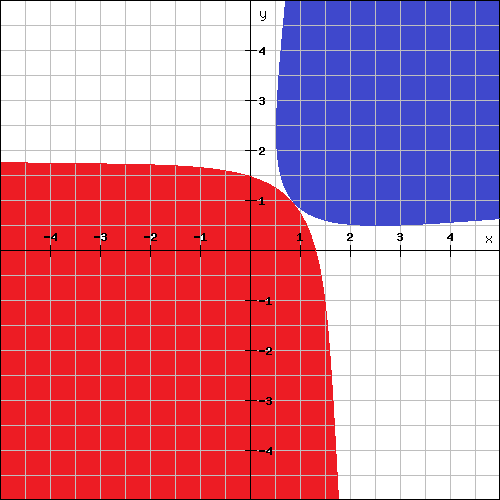
\includegraphics{SAT-touching.png} 
\caption{SAT(UNSAT) detected by Grobner basis method} 
\label{fig:sat-touching} 
%\end{minipage}
\end{figure} 

\item \textbf{UNSAT without touching/convergence}
\begin{figure}[ht]
%\begin{minipage}[b]{1.0\linewidth}
\centering
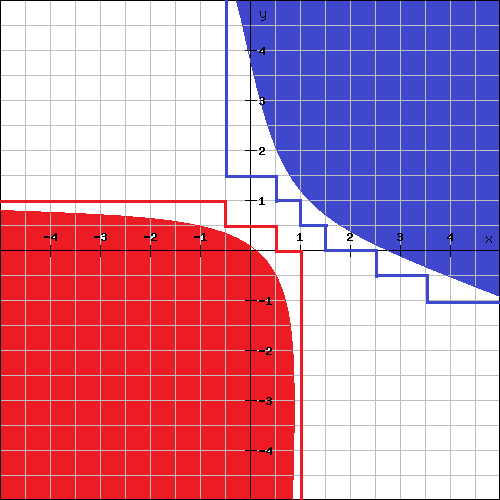
\includegraphics{UNSAT-withoutTouching.png} 
\caption{UNSAT detected by ICP} 
\label{fig:unsat-withoutTouching} 
%\end{minipage}
\end{figure} 
\end{enumerate}
\end{comment}
\begin{comment}
$\exists x_1 \in (a_1,b_1) \cdots x_n \in (a_n,b_n) . \wedge_{i} f_i > 0$, 
\begin{itemize}
\item If $\exists x_1 \in (a_1,b_1) \cdots x_n \in (a_n,b_n) . \wedge_{i} f_i > 0$ is SAT, 
ICP eventually detects it. 
\item If $\exists x_1 \in [a_1,b_1] \cdots x_n \in [a_n,b_n] . \wedge_{i} f_i \geq 0$ is UNSAT, 
ICP eventually detects it
\end{itemize}
under the assumptions of {\em fair} decomposition and bounded intervals. 
\begin{figure}[ht]
%\begin{minipage}[b]{1.0\linewidth}
\centering
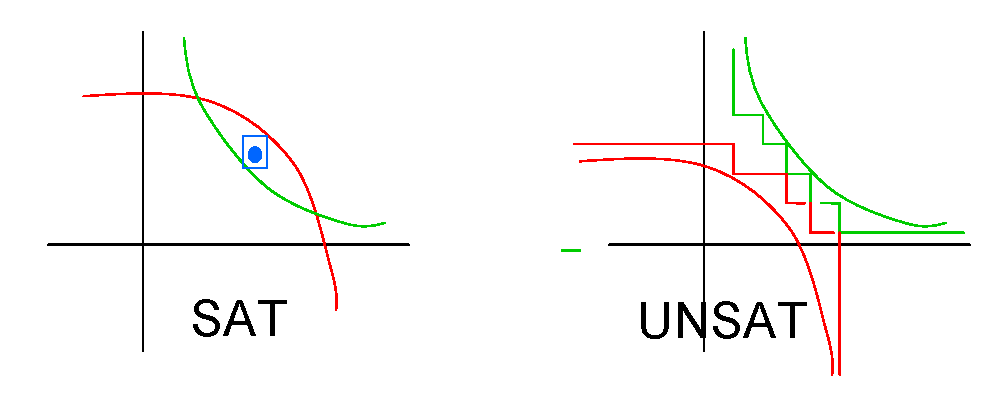
\includegraphics[height=1.2in,width=3.4in]{FigCompleteness.eps} 
\caption{SAT and UNSAT detection by ICP} 
\label{fig:complete} 
%\end{minipage}
\end{figure} 

The boundary part is reduced to polynomial equality checking, 
which would be solved algebraic methods, like Groebner basis. 
Alternatively, by loosening equality to $\delta$-equality, 
$\delta$-completeness is obtained~\cite{dRealIJCAR12,dRealLICS12}. 

This paper presents an SMT solver {\bf raSAT} for polynomial inequality. 
It consists of a simple iterative approximation refinement, called {\bf raSAT} {\em loop}, 
which is an extension of the standard ICP with testing to accelerate SAT detection. 
Two approximation schemes consist of interval arithmetic (over-approximation) and 
testing (under-approximation), to accelerate SAT detection. 
If both fails, input intervals are refined by decomposition. 
%
Compared to typical ICPs, {\bf raSAT} 
\begin{itemize}
\item introduces testing (as an under-approximation) to accelerate SAT detection, 
\item applies various interval arithmetic, e.g., Affine intervals~\cite{Stolfi03,ngocase,tapas12}, 
which enables to analyze the effects of input values, and 
\item SAT confirmation step by an error-bound guaranteed floating point package {\bf iRRAM}\footnote{% 
\tt http://irram.uni-trier.de}, to avoid soundess bugs caused by roundoff errors. 
\end{itemize}
This design is more on SAT detection oriented, since from our preliminary experiences, 
if the target problems have several hundred variables, solvable cases in practice are 
either SAT or UNSAT with small UNSAT core. 
Thus, acceleration of SAT detection and finding UNSAT core will be keys for scalability. 

ICP is robust for larger degrees, but the number of boxes (products of intervals) to explore 
exponentially explodes when variables increase. 
Thus, design of strategies for selecting variables to decompose and boxes to explore is crucial 
for efficiency. Our strategy design is, 
\begin{itemize}
\item a box with more possiblity to be SAT is selected to explore, which is estimated by 
several heuristic measures, called {\em SAT likelyhood}, 
and the number of unsolved atomic polynomial constraints, and
\item a more influential variable is selected for multiple test cases and decomposition, 
which is estimated by {\em sensitivity}. 
\end{itemize} 
Note that {\em SAT likelyhood} and {\em sensitivity} are estimated during interval arithmetic. 
Especially, the latter can be applied only with Affine intervals. 
{\bf raSAT} also applies incremental search, which is often faster in practice. 
\begin{itemize}
\item {\bf Incremental widening}. 
Starting {\bf raSAT} loop with a smaller interval, and if it is UNSAT, enlarge the input intervals
and restart. 
\item {\bf Incremental deepening}. 
Starting with the bound that each interval will be decomposed no smaller than it. 
If neither SAT nor UNSAT is detected, take a smaller bound and restart. 
\end{itemize} 
Efficient UNSAT core and UNSAT confirmation % with error bound guaranteed floating point arithmetic 
are left for future work. 

They are compared on Zankl and Meti-Tarski benchmarks from 
QF\_NRA category of SMT-LIB\footnote{\tt http://www.smtlib.org/}. 
They are also evaluated by comparing 
{\bf Z3 4.3}\footnote{\tt http://z3.codeplex.com} and {\bf iSAT3}. 
Another advantage of {\bf raSAT} is the ease to handle mixed intergers, 
and experiments on AProVE benchmark from QF\_NIA category of SMT-LIB compares {\bf raSAT} with 
{\bf Z3 4.3}. 
Although {\bf Z3 4.3} performs the best, {\bf raSAT} shows comparable SAT detection on 
very large problems (e.g., with several hundred variables) with the combination of 
{\em SAT likelyhood} and {\em sensitivity}. 


\medskip 
{\bf raSAT} applies SAT confirmation to avoid soundness errors caused by roundoff/overflow errors. 
Another static analysis based approach is found in~\cite{SilvaTACAS12}. 
\end{comment}

\section{Thesis outline}
Coming soon...

\chapter{Preliminaries}
\section{Abstract DPLL}
\section{SMT}
\section{Polynomial constraints}
A polynomial is formally defined as:
\begin{center}
\begin{grammar}
<polynomial> ::= 1 | <variable> | rational\_constant 
				 \alt polynomial + polynomial
			     \alt polynomial - polynomial
			     \alt polynomial * polynomial
\end{grammar}
\end{center}

\chapter{Over-Approximation and Under-Approximation for Polynomials}
This section presents Interval Arithmetic as an over-approximation theory, and testing as an under-approximation theory.

\chapter{Interval Arithmetic}
Interval Arithmetic is defined formally in Section ~\ref{sec:IA} of Chapter ~\ref{chap:OT-UT}. This chapter is going to present two instances of Interval Arithmetic which are used in raSAT: Classical Interval and Affine Interval. These two kinds differ to each other in the way they represent intervals and interpret function symbols.

\section{Classical Interval}
A model $M^p_{CI} = (U^p_{CI}, I^p_{CI})$ over intervals contains a set of all intervals $U^p_{CI} = U^p_{IA}$ and a map $I^p_{CI}$ that satisfies the following conditions.
\begin{enumerate}
\item $I^p_{CI}(Real) = I^p_{IA}(Real)$
\item $\forall p \in P^p$; $I^p_{CI}(p)= I^p_{IA}(p)$
\item $\forall f \in F^p \setminus \{\mathbf{1}\}$; $I^p_{CI}(f) = U^p_{CI} \times U^p_{CI} \mapsto U^p_{CI}$ such that $ I^p_{CI}(f)(i_1, i_2)= i_1 \; f_{CI} \; i_2$ where the definition of $f_{CI}$ is:
\begin{itemize}
\item $\langle l_1, h_1 \rangle \oplus_{CI} \langle l_2, h_2 \rangle = \langle l_1 + l_2, h_1 + h_2 \rangle $.
\item $\langle l_1, h_1 \rangle \ominus_{CI} \langle l_2, h_2 \rangle = \langle l_1 - h_2, h_1 - l_2 \rangle $.
\item Operation $i_1 \otimes_{CI} i_2$ is defined using case analysis on the types of $i_1$ and $i_2$. First, the intervals are classified into the following:
\begin{itemize}
\item $P = \{\langle a, b \rangle | a \ge 0 \wedge b > 0 \}$
\item $N = \{\langle a, b \rangle | b \le 0 \wedge a < 0 \}$
\item $M = \{\langle a, b \rangle | a < 0 < b \}$
\item $Z = \{\langle a, b \rangle\}$
The definition of $\otimes_{CI}$ is given in Table ~
\begin{center}
\begin{tabular}{ | c | c | c |}
\hline
Class of $\langle l_1, h_1 \rangle$ & Class of $\langle l_2, h_2 \rangle$ & $\langle l_1, h_1 \rangle \otimes_{CI} \langle l_2, h_2 \rangle$ \\ \hline
P & P & $\langle l_1 \times l_2, h_1 \times h_2 \rangle $ \\ \hline
P & M & $\langle h_1 \times l_2, h_1 \times h_2 \rangle $ \\ \hline
P & N & $\langle h_1 \times l_2, l_1 \times h_2 \rangle $ \\ \hline
M & P & $\langle l_1 \times h_2, h_1 \times h_2 \rangle $ \\ \hline
M & M & $\langle \min (l_1 \times h_2, h_1 \times l_2), max (l_1 \times l_2, h_1 \times h_2) \rangle $ \\ \hline
M & N & $\langle h_1 \times l_2, l_1 \times l_2 \rangle $ \\ \hline
N & P & $\langle l_1 \times h_2, h_1 \times l_2 \rangle $ \\ \hline
N & M & $\langle l_1 \times h_2, l_1 \times l_2 \rangle $ \\ \hline
N & N & $\langle h_1 \times h_2, l_1 \times l_2 \rangle $ \\ \hline
Z & P, N, M, Z & $\langle 0, 0 \rangle $ \\ \hline
P, N, M & Z & $\langle 0, 0 \rangle $ \\ \hline
\end{tabular}
\end{center}
\end{itemize}

\end{itemize}
\item $I^p_{CI}(\mathbf{1}) = \langle 1,1\rangle $
\item $\forall v \in V$; $I^p_{CI} \in U^p_{CI}$
\end{enumerate}
Theory $T^p_{CI} = \{M^p_{CI}| M^p_{CI} \text{ is a model over intervals}\}$. Each model differs to another by the mapping from variables to intervals. As a consequence, one assignment from variables to intervals can be used to describe an model. We denote $\Pi^p_{CI}$ as the model represented by $\Pi = \{x \in \langle l, h\rangle  | v \in V\}$. 
\begin{theorem}
CI is an IA.
\end{theorem}
\begin{proof}
Easy.
\end{proof}
\section{Affine Interval}
Affine Interval use the formula $a_0 + \sum\limits_{i=1}^{n} a_i\epsilon_i$ to represent the interval $\langle a_0 - \sum\limits_{i=1}^{n}|a_i|, a_0 + \sum\limits_{i=1}^{n}|a_i| \rangle$ with $a_i \in \mathbb{R}$ for $i = 0, 1, \cdots$. For example, the affine interval form of $(x \in) \langle 2, 4 \rangle$ and $(y \in) \langle 0, 2 \rangle$ is $3 + \epsilon_1$ and $1 + \epsilon_2$ respectively, thus:

\begin{center}
$\begin{aligned}[t]
    x^2 - x \times y  &= (3 + \epsilon_1)^2 - (3 + \epsilon_1) \times (1 + \epsilon_2)\\
     &= 9 + 6\epsilon_1 + \epsilon_1^2- (3 + 3\epsilon_2 + \epsilon_1 + \epsilon_1\epsilon_2) \\
     &= 6 + 5\epsilon_1 - 3\epsilon_2 + \epsilon_1^2 + \epsilon_1\epsilon_2
\end{aligned}$
\end{center}
Types of affine interval vary by choices of estimating multiplications $\epsilon_1^2$ and $\epsilon_1\epsilon_2$:
\begin{enumerate}
\item AA \cite{Comba93affinearithmetic, Stolfi97self-validatednumerical} replaces $\epsilon_1\epsilon_2$ by a fresh noise symbol. 
\item AF1 and AF2 \cite{Messine_extensionsof} prepares a fixed noise symbol for any $\epsilon_1\epsilon_2$.
\item EAI \cite{Ngoc:2009:ORE:1685167.1685421} replaces $\epsilon_1\epsilon_2$ by $\langle -1, 1 \rangle\epsilon_1$ or $\langle -1, 1 \rangle\epsilon_2$.
\item AF2 \cite{Messine_extensionsof} replaces $\epsilon_1^2$ by the fixed noise symbols $\epsilon_+$ or $\epsilon_-$.
\end{enumerate}
A model $M^p_{AF2} = (U^p_{AF2}, I^p_{AF2})$ over intervals contains a set of all intervals $U^p_{AF2} = \{a_0 + \sum\limits_{i=1}^{n}a_i\epsilon_i + a_{n+1}\epsilon_+ + a_{n+2}\epsilon_- + a_{n+3}\epsilon_{\pm} | \forall i \in \{0, 1, \cdots, n+3\}; a_i \in \mathbb{R}\}$ and a map $I^p_{AF2}$ that satisfies the following conditions.
\begin{enumerate}
\item $I^p_{AF2}(Real) = U^p_{AF2}$
\item $\forall p \in P^p$; $I^p_{AF2}(p)= U^p_{AF2} \times U^p_{AF2} \mapsto \{true, false\}$ such that $I^p_{AF2}(p)(a_0 + \sum\limits_{i=1}^{n}a_i\epsilon_i + a_{n+1}\epsilon_+ + a_{n+2}\epsilon_- + a_{n+3}\epsilon_{\pm}, b_0 + \sum\limits_{i=1}^{n}b_i\epsilon_i + b_{n+1}\epsilon_+ + b_{n+2}\epsilon_- + b_{n+3}\epsilon_{\pm}) = I^p_{AI}(p)(\langle a_0 - \sum\limits_{i=1}^{n}|a_i| - a_{n+2} - a_{n+3}, a_0 + \sum\limits_{i=1}^{n}|a_i| + a_{n+1} + a_{n+3} \rangle, \langle b_0 - \sum\limits_{i=1}^{n}|b_i| - b_{n+2} - b_{n+3}, b_0 + \sum\limits_{i=1}^{n}|b_i| + b_{n+1} + b_{n+3} \rangle)$
\item $\forall f \in F^p \setminus \{\mathbf{1}\}$; $I^p_{AF2}(f) = U^p_{AF2} \times U^p_{AF2} \mapsto U^p_{AF2}$ such that $ I^p_{AF2}(f)(i_1, i_2)= i_1 \; f_{AF2} \; i_2$ where the definition of $f_{AF2}$ is as following. Let $i_1 = a_0 + \sum\limits_{i=1}^{n}a_i\epsilon_i + a_{n+1}\epsilon_+ + a_{n+2}\epsilon_- + a_{n+3}\epsilon_{\pm}$ and $i_2 = b_0 + \sum\limits_{i=1}^{n}b_i\epsilon_i + b_{n+1}\epsilon_+ + b_{n+2}\epsilon_- + b_{n+3}\epsilon_{\pm}$, then:
\begin{itemize}
\item $i_1 \oplus_{AF2} i_2 = a_0 + b_0 + \sum\limits_{i=1}^{n}(a_i + b_i)\epsilon_i + (a_{n+1} + b_{n+1})\epsilon_+ + (a_{n+2} + b_{n+2})\epsilon_- + (a_{n+3} + b_{n+3})\epsilon_\pm$.
\item $i_1 \ominus_{AF2} i_2 = a_0 - b_0 + \sum\limits_{i=1}^{n}(a_i - b_i)\epsilon_i + (a_{n+1} + b_{n+1})\epsilon_+ + (a_{n+2} + b_{n+2})\epsilon_- + (a_{n+3} + b_{n+3})\epsilon_\pm$.
\item $i_1 \otimes_{AF2} i_2 = a_0b_0 + \sum\limits_{i=1}^{n}(a_0b_i + a_ib_0)\epsilon_i + K_1\epsilon_+ + K_2\epsilon_-  + K_3\epsilon_\pm$, where:

$K_1 = \sum\limits_{i=1,a_ib_i>0}^{n+3}a_ib_i + \left\{ 
  \begin{array}{l l}
    a_0b_{n+1} + a_{n+1}b_0 & \quad \text{if } a_0 \ge 0 \text{ and } b_0 \ge 0\\
    a_0b_{n+1} - a_{n+2}b_0 & \quad \text{if } a_0 \ge 0 \text{ and } b_0 < 0\\
    -a_0b_{n+2} + a_{n+1}b_0 & \quad \text{if } a_0 < 0 \text{ and } b_0 \ge 0\\
    -a_0b_{n+2} - a_{n+2}b_0 & \quad \text{if } a_0 < 0 \text{ and } b_0 < 0\\
  \end{array} \right.$
  
$K_2 = \sum\limits_{i=1,a_ib_i<0}^{n+3}a_ib_i + \left\{ 
  \begin{array}{l l}
    a_0b_{n+2} + a_{n+2}b_0 & \quad \text{if } a_0 \ge 0 \text{ and } b_0 \ge 0\\
    a_0b_{n+2} - a_{n+1}b_0 & \quad \text{if } a_0 \ge 0 \text{ and } b_0 < 0\\
    -a_0b_{n+1} + a_{n+2}b_0 & \quad \text{if } a_0 < 0 \text{ and } b_0 \ge 0\\
    -a_0b_{n+1} - a_{n+1}b_0 & \quad \text{if } a_0 < 0 \text{ and } b_0 < 0\\
  \end{array} \right.$  

$K_3 = \sum\limits_{i=1}^{n+3}\sum\limits_{j=1,j \neq i}^{n+3}|a_ib_j| + |a_0|b_{n+3} + a_{n+3}|b_0|$
\end{itemize}
\item $I^p_{AF2}(\mathbf{1}) = 1$
\item $\forall v \in V$; $I^p_{AF2} \in U^p_{AF2}$
\end{enumerate}
Theory $T^p_{AF2} = \{M^p_{AF2}| M^p_{AF2} \text{ is a model over intervals}\}$. Each model differs to another by the mapping from variables to intervals. As a consequence, one assignment from variables to intervals can be used to describe an model. We denote $\Pi^p_{CI}$ as the model represented by $\Pi = \{x \in \langle l, h\rangle  | v \in V\}$. 
\begin{theorem}
AI is an IA.
\end{theorem}
\begin{proof}
Easy.
\end{proof}

\begin{comment}
We design an SMT solver named raSAT~\footnote{\url{http://www.jaist.ac.jp/~mizuhito/tools/rasat.html}} to solve polynomial constraint. 

Although an $O.T$ refinement loop is enough to implement an ICP based SMT solver, 
we extend it as {\bf raSAT} (SAT by refinement of approximations) loop to accelerate SAT detection 
by adding $U.T$, which works as in Fig.~\ref{fig:OTrefine}~(b). 
\begin{enumerate}
\item When an over-approximation theory $O.T$ detects $O.T$-UNSAT (resp. $O.T$-valid), 
answer UNSAT (resp. SAT). 
\item When an under-approximation theory $U.T$ detects $U.T$-SAT, answer SAT. 
\item If neither holds, a refinement is applied. 
\end{enumerate}

Our design of an SMT solver {\bf raSAT} applies two heuristic features. 
\begin{itemize}
\item Incremental widening intervals, and incremental deeping search 
(Section~\ref{sec:incsearch}). 
\item 
Heurstic measures {\em SAT-likelyhood} and {\em sensitivity}, 
for selection of a variable to decompose and a box to explore. 
(Section~\ref{sec:SATheuristics}). 
\end{itemize} 

{\bf raSAT} also prepares various interval arithmetic as $O.T$ as in Section~\ref{sec:approximation}, 
whereas currently only random tesing (\emph{k-random ticks}, 
which consists of periodical $k$-test instances with a random offset) is prepared as $U.T$. 

A typical theory for $O.T$ and $U.T$ are an interval arithmetic and testing, respectively. 
We say {\em IA-valid}, {\em IA-SAT}, and {\em IA-UNSAT}, when it is $O.T$-valid, $O.T$-SAT, and 
$O.T$-UNSAT, respectively. 
Similarly, we say {\em test-SAT} and {\em test-UNSAT}, when it is $U.T$-SAT and $U.T$-UNSAT, respectively. 
Note that either IA-valid or test-SAT implies SAT, and IA-UNSAT implies UNSAT, 
whereas IA-SAT and test-UNSAT can conclude neither. 


%We instantiate testing to $U.T$ in Section~\ref{sec:raSATloop}. 
%%%%%%%%%%%%%%%%
\suppress{
\begin{definition}\label{def:testing}
%For $\exists x_1 \in (a_1,b_1) \cdots x_n \in (a_n,b_n). \bigwedge \limits_{i=1}^m f_i(x_1,\cdots,x_n) > 0$, 
Let $M = \bigwedge \limits_{i=1}^m x_i \in (a_i,b_i)$ and 
${\mathcal P} = \bigwedge \limits_{i=1}^m f_i(x_1,\cdots,x_n) > 0$. 
%
Let a choice function $\theta : (\Real \times \Real)^n \rightarrow \Real^n$ 
such that $\theta(M) \in (a_1,b_1) \times \cdots \times (a_n,b_n)$. 
Testing is a finite set $\Theta$ of choice functions. Then, we say 
\begin{itemize}
\item ${\mathcal P}$ is \emph{Test-SAT} under $M$ if $\theta(M)$ holds ${\mathcal P}$ 
for some $\theta \in \Theta$, and 
\item ${\mathcal P}$ is \emph{Test-UNSAT} under $M$ if $\theta(M)$ never holds ${\mathcal P}$ 
for each $\theta \in \Theta$. 
\end{itemize} 
%We denote $I \models_{test(\theta)} P$ if $\bigwedge \limits_{i=1}^m f_i(\theta(I)) > 0$ holds.
\end{definition}
}
%%%%%%%%%%%%%%%%


{\bf raSAT} prepares various Affine intervals, adding to classical interval (CI)~\cite{moore}, 
which keep lower and upper bounds. The weakness of CI is loss of dependency 
among values. For instance, $x - x$ is evaluated to $(-2,2)$ for $x \in (2,4)$. 

Affine Interval~\cite{af,comba93} introduces \emph{noise symbols} $\epsilon$, 
which are interpreted as values in $(-1,1)$. 
For instance, $x = 3 + \epsilon$ describes $x \in (2,4)$, and 
$x - x = (3 + \epsilon) - (3 + \epsilon)$ is evaluated to $0$. 
The drawback is that the multiplication without dependency might be less precise than CI.
Affine intervals also cannot represent infinite intervals, e.g., $(0,\infty)$, 
since it becomes $\infty + \infty~\epsilon$. 
Forms of affine intervals vary by choices how to approximate multiplications. They are,
\begin{enumerate}[(i)]
\item $\epsilon \epsilon'$ is replaced with a fresh noise symbol 
($AF$)~\cite{StolfiThesis,comba93}, 
\item $\epsilon \epsilon'$ is reduced to the fixed error noise symbol 
$\epsilon_{\pm}$ ($AF_1$ and $AF_2$) \cite{af},
\item $\epsilon \epsilon'$ is replaced with $(-1,1) \epsilon$ 
(or $(-1,1) \epsilon'$) ($EAI$)~\cite{ngocsefm},
\item $\epsilon \epsilon$ is reduced to fixed noise symbols 
$\epsilon_+$ or $\epsilon_{-}$ ($AF_2$) \cite{af}, 
\item Chebyshev approximation of $x^2$ introduces a noise symbol $|\epsilon|$ 
as an absolute value of $\epsilon$ with 
$\epsilon \epsilon = |\epsilon| |\epsilon| = |\epsilon| + (-\frac{1}{4}, 0)$ and
$\epsilon |\epsilon| = \epsilon + (-\frac{1}{4}, \frac{1}{4})$ \cite{tapas12}. 
%(Fig.~\ref{fig:chevabs}). 
%\item keeping products of noise symbols up to degree $2$ ($\epsilon_i \epsilon_j$),
\end{enumerate} 

%%%%%%%%%%%%%%%%%
\suppress{
\begin{remark}
For Affine intervals, \emph{sensitivity}~\cite{ngocsefm} of a variable
is a possible range of the absolute value of the coefficient of its corresponding $\epsilon$. 

%In Example~\ref{examp:sensitivity}, $CAI$ estimates the coefficient of $|\epsilon_1|$ as $\textbf{3}$, 
%which has the largest sensitivity and indicates $x$ the most influencial. 

Note that Affine interval works only for bounded intervals. 
For instance, $\infty + \infty \epsilon$ represents $(-\infty,\infty)$, which says nothing. 
Narrowing intervals as an incremental search (Section~\ref{sec:incsearch}) partilly depends on this fact. 
That is, if $\pm \infty$ is contained in an interval, first give finite upper/lower bounds and search 
within these bounds using an Affine interval. If UNSAT is concluded, then enlarge to the whole intervals 
using CI. 
\end{remark}
}
%%%%%%%%%%%%%%%%%


\begin{example} \label{examp:sensitivity}
Let $f = x^3 - 2xy$ with $x = (0,2)$ ($x = 1 + \epsilon_1$) and $y=(1,3)$ ($y = 2+\epsilon_2$), 
we have,
\begin{itemize}
\item $AF_2$ estimates the range of $f$ as 
$-3 - \epsilon_1 - 2\epsilon_2 + 3\epsilon_+ + 3\epsilon_{\pm}$, thus $(-9,6)$,
\item $CAI$ estimates the range of $f$ as 
$(-4,-\frac{11}{4}) + (-\frac{1}{4}, 0)\epsilon_1 - 2\epsilon_2 + \textbf{3}|\epsilon_1| + (-2,2)\epsilon_{\pm}$, 
thus $(-8,4.5)$.
\end{itemize}
\end{example}



%%%%%%%%%%%%%%%%%%%%%%%%%%
\suppress{
\begin{figure}[ht]
\begin{minipage}[b]{1.0\linewidth}
\centering
\begin{tabular}{ll}
\includegraphics[height=1.6in,width=1.7in]{chev1.pdf} &
\includegraphics[height=1.6in,width=1.7in]{chev2.pdf}
\end{tabular}
\caption{Chebyshev approximation of $x^2$ and $x~|x|$}
\label{fig:chevabs}
\end{minipage}
\end{figure}

$CAI$ \cite{tapas12} consists of (ii) and (v), which keeps better precision than iv)
for multiplicatins of the same variables, e.g., Taylor expansion. 
%To improve precision in estimating upper and lower bounds of polynomials, we apply 
%\textbf{Affine Arithmetic} such as $AF_1$, $AF_2$ \cite{af}, $CAI$ ~\cite{tapas12} 
%instead of Classical Interval \cite{moore}. 
%Note that upper and lower bounds estimated by IA are over-approximation bounds of polynomials.

}
%%%%%%%%%%%%%%%%%%%%%%%%%%
\suppress{
\begin{definition}
%For $\exists x_1 \in (a_1,b_1) \cdots x_n \in (a_n,b_n). \bigwedge \limits_{i=1}^m f_i(x_1,\cdots,x_n) > 0$, 
Let $M = \bigwedge \limits_{i=1}^m x_i \in (a_i,b_i)$ and 
${\mathcal P} = \bigwedge \limits_{i=1}^m f_i(x_1,\cdots,x_n) > 0$. 
%
Let $\delta_i^l$ and $\delta_i^u$ be lower and upper bounds of $f_i(x_1,\cdots,x_n)$ 
estimated by IA for $x_i \in (a_i,b_i)$. Then, we say 
%
%\vspace*{0.5em}
\begin{itemize}
\item ${\mathcal P}$ is \emph{IA-VALID} under $M$, if IA evaluates 
$~\forall i \in [1,m].~\delta_i^l > 0$,
%\vspace*{0.33em}
\item ${\mathcal P}$ is \emph{IA-UNSAT} under $M$, 
$~\exists i \in [1,m].~\delta_i^u \leq 0$, and 
\item ${\mathcal P}$ is \emph{IA-SAT} under $M$, if 
$(\exists j \in [1,m].~\delta_j^l \leq 0)\; \wedge \; 
	(\bigwedge \limits_{i=1}^m \delta_i^u > 0)$.
\end{itemize} 
\end{definition}

IA-VALID and IA-UNSAT safely reason satisfiability (SAT) and unsatisfiability (UNSAT), 
respectively. However, IA-SAT cannot conclude SAT. 
}


\suppress{
I. Selecting API for testing:
  (1) Difficulty first by SAT-likelihood.   
  (2) Easy first by SAT-likelihood
  (10) Random.,
II. Selecting Variable:
  (8) With sensitivity
  (9) Without sensitivity - Random: 
III. Selecting box:
  (3) SAT-directed using IA-Testing.
  (4) UNSAT-directed using IA-Testing.
  (5) SAT-directed using SAT-likelihood
  (6) UNSAT-directed using SAT-likelihood
  (7) Random
}
\end{comment} 


\chapter{Design strategies}
We implemented a number of strategies for improving efficiency of raSAT: incremental search and refinement heuristics.
\section{Incremental search} \label{sec:incsearch}
{\bf raSAT} applies three incremental strategies, 
(1) {\em incremental windening}, (2) {\em incremental deepening} and (3) {\em incremental testing}. 
Let
$F = \exists x_1 \in I_1 \cdots x_n \in I_n. \bigwedge \limits_{j=1}^m f_j > 0$
for $I_i = (a_i,b_i)$. %where $a_i, b_i$ would be $\pm \infty$. 

\subsection{Incremental windening}
Given $0 < \delta_0 < \delta_1 < \cdots$, 
{\em incremental windening} starts with 
$F_0 = \exists x_1 \in I_1 \cap (-\delta_0 , \delta_0) \cdots x_n \in I_n \cap (-\delta_0 , \delta_0). 
\bigwedge \limits_{j=1}^m f_j > 0$, 
and if it finishes with UNSAT, it runs with 
$F_1 = \exists x_1 \in I_1 \cap (-\delta_1 , \delta_1) \cdots x_n \in I_n \cap (-\delta_1 , \delta_1). 
\bigwedge \limits_{j=1}^m f_j > 0$, and so on (Fig.~\ref{fig:incwid} (a)). 

Note that if $\delta_i < \infty$, {\bf raSAT} applies an Affine interval; otherwise, 
it uses CI. 
Experiments in Section~\ref{sec:experiment} are performed 
with $\delta_0 = 10$ and $\delta_1 = \infty$.
\begin{figure}[ht]
\begin{minipage}[b]{1.0\linewidth}
\centering
\begin{tabular}{c@{\qquad}c}
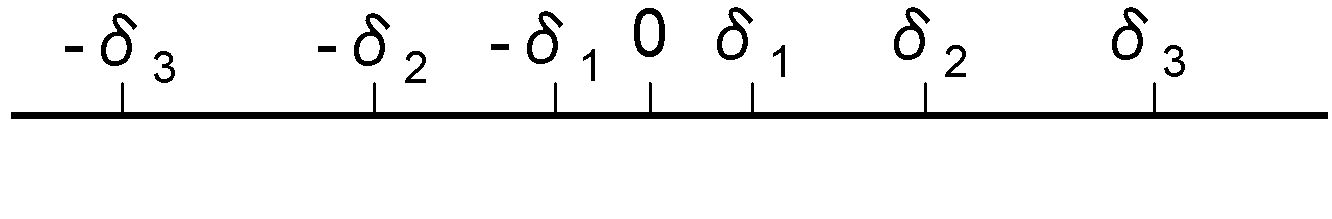
\includegraphics[height=0.4in,width=1.8in]{IncWiden.png} &
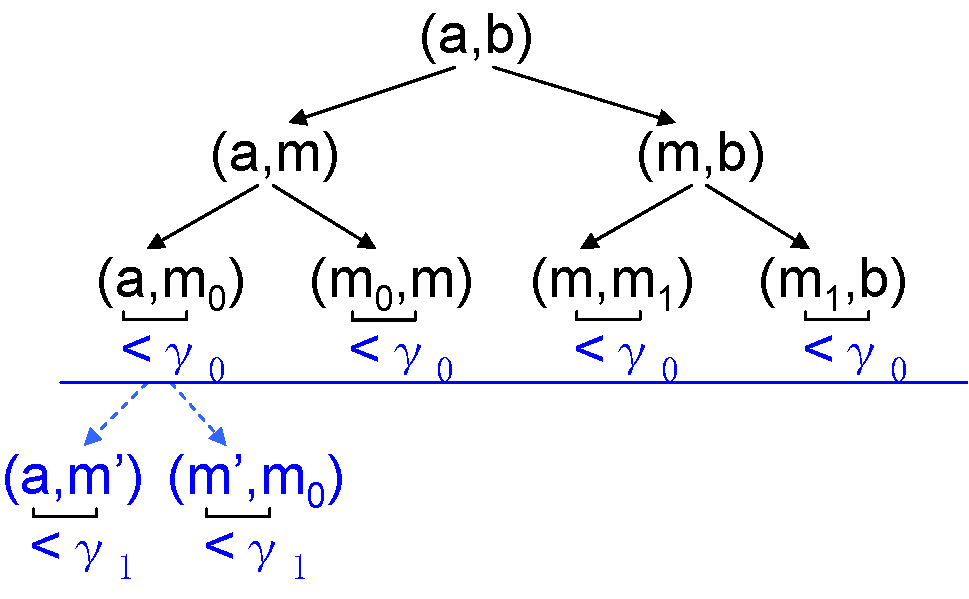
\includegraphics[height=1.2in,width=2in]{IncDeepen.png} \\
\mbox{(a) Incremenal widening} & \mbox{(b) Incremental Deepening} \\
\end{tabular}
\caption{Incremental Widening and Deepening}
\label{fig:incwid}
\end{minipage}
\end{figure}


\subsection{Incremental deepening}

Starting with $F = \exists x_1 \in I_1 \cdots x_n \in I_n. \bigwedge \limits_{j=1}^m f_j > 0$, 
$I_1 \times \cdots \times I_n$ is decomposed into many boxes, 
and $F$ becomes the disjunction of existential formulae corrsponding to these boxes. 
{\bf raSAT} searches these boxes in depth-first manner, which may leads to local optimal search. 
To avoid it, {\bf raSAT} applies a threshold $\gamma$, such that no more decomposition will be 
applied when a box becomes smaller than $\gamma$. 
If neither SAT nor UNSAT is detected, {\bf raSAT} restarts with a smaller threshhold. 

Let $\gamma_0 > \gamma_1 > \cdots > 0$, and {\bf raSAT} incrementally deepens its search 
with these threshholds, i.e., starting with $\delta_0$, and if it fails, restart with $\delta_1$, 
and so on (Fig~\ref{fig:incwid} (b)). 

\section{SAT directed heuristics measure} \label{sec:SATheuristics}

With several hundred variables, we observe that an SMT solver works 
when either SAT, or UNSAT with small UNSAT core.
%
For the latter, we need an efficient heuristics to find an UNSAT core, which is left as future work. 
For the former, the keys are how to choose variables to decompose, and 
how to choose a box to explore. 
{\bf raSAT} chooses such a variable in two steps; first it selects a {\em test-UNSAT API}, and
then chooses a variable that appears in the API. 
We design SAT-directed heuristic measures based on the interval arithemtic ($O.T$). 

Let $F = \exists x_1 \in I_1 \cdots x_n \in I_n. \bigwedge \limits_{j=1}^m f_j > 0$ 
becomes $\vee~( \exists x_1 \in I'_1 \cdots x_n \in I'_n. \bigwedge \limits_{j=1}^m f_j > 0)$ 
after box decomposition. 
For $\exists x_1 \in I'_1 \cdots x_n \in I'_n. \bigwedge \limits_{j=1}^m f_j > 0$, 
if some $f_j > 0$ is UNSAT, the box $I'_1 \times \cdots \times I'_n$ is UNSAT. 
If every $f_j > 0$ is SAT, $F$ is SAT. 
Thus, if the box $I'_1 \times \cdots \times I'_n$ needs to be explore, it must contain 
a test-UNSAT API (thus IA-SAT). 

We denote the estimated range of $f_j$ for $x_1 \in I'_1 \cdots x_n \in I'_n$ with IA ($O.T$)
by $range(f_j, I'_1 \times \cdots \times I'_n)$. 
If an IA is an affine interval, 
it is in the form $[c_1,d_1]\epsilon_1 + \cdots + [c_n,d_n]\epsilon_n$, 
and by instanciating $\epsilon_i$ with $[-1,1]$, 
the resulting classical interval coincides with $range(f_j, I'_1 \times \cdots \times I'_n)$. 
We define 
\begin{itemize} 
\item {\em Sensitivity} of a variable $x_i$ in a test-UNSAT API $f_j > 0$ is $max(|c_i|, |d_i|)$. 
\item {\em SAT-likelyhood} of an API $f_j > 0$ is $| I \cap (0,\infty) | / |I|$, and 
\item {\em SAT-likelyhood} of a box $I'_1 \times \cdots \times I'_n$ is 
the least SAT-likelyhood of test-UNSAT APIs. 
\end{itemize} 

\begin{example} \label{examp:SATlikelyhood}
In Example~\ref{examp:sensitivity}, 
\begin{itemize}
\item sensitivity is estimated $1$ for $x$ and $2$ for $y$ by $AF_2$, and $3\frac{1}{4}$ for $x$ and 
$2$ for $y$. 
\item SAT-likelyhood of $f$ is estimated $0.4= \frac{6}{9-(-6)}$ by $AF_2$ 
and $0.36 = \frac{4.5}{4.5-(-8)}$ by $CAI$. 
\end{itemize}
\end{example}


{\em SAT-likelyhood} intends to estimate APIs how likely to be SAT. 
For choosing variables, {\bf raSAT} first choose a test-UNSAT API by SAT-likelyhood. 
There are two choices, either {\em the largest} or {\em the least}. 
{\em Sensitivity} of a variable intends to estimate how a variable is influencial to the value of an API. 
From a selected API by SAT-likelyhood, {\bf raSAT} selects a variable with the largest sensitivity. 
This selection of variables are used for (1) {\em multiple test instances generation}, and 
(2) {\em decomposition}. 
For test generation, we will select multiple variables by repeating the selection. 

For choosing a box to explore, {\bf raSAT} chooses more likely to be SAT. 
There are two choice, (1) a box with the largest SAT-likelyhood, and 
(2) a box with the largest number of SAT (either IA-valid or test-SAT) APIs. 

\chapter{Experiments}
This chapter is going to present the experiments results which reflect how effective our designed strategies are. In addition, comparison between raSAT, Z3 and iSAT3 will be also shown. The experiments were done on a system with  Intel Xeon E5-2680v2 2.80GHz and 4 GB of RAM. In the experiments, we exclude the problems which contain equalities because currently raSAT focuses on inequalities only.

\section{Experiments on strategy combinations} \label{sec:expstrategy}

We perform experiments only on Zankl, and Meti-Tarski families. 


Our combinations of strategies mentioned in Section~\ref{sec:strategy} are, 

\medskip
{\centering
\begin{tabular}{l|l|l}
Selecting a test-UNSAT API~~ & Selecting a box (to explore): & 
Selcting a variable: \\  % (for testing and decomposition)
\hline

(1) Least SAT-likelyhood. & 
(3) Largest number of SAT APIs.~~ & 
(8) Largest sensitibity. \\

(2) Largest SAT-likelyhood. & 
(4) Least number of SAT APIs. & \\

& (5) Largest SAT-likelyhood. & \\

& (6) Least SAT-likelyhood. & \\

(10) Random. & (7) Random. & (9) Random. \\
\end{tabular}
}
\medskip

Table~\ref{tab:rasat-experiments} shows the experimental results of above mentioned combination. 
The timeout is set to 500s, and each time is the total of successful cases 
(either SAT or UNSAT). 

Note that (10)-(7)-(9) means all random selection. 
Generally speaking, the combination of (5) and (8) show the best results, 
though the choice of (1),(2), and (10) shows different behavior on benchmarks. 
We tentatively prefer (1) or (10), but it needs to be investigated further. 

\begin{table*}[t]
\centering
\begin{tabular}{ | l | r | r  r | r | r  | r | r | r | r | r | r |r | r |}
\hline
    \multicolumn{1}{|l|}{Benchmark} & 
    \multicolumn{3}{c|}{(1)-(5)-(8)} & \multicolumn{2}{c|}{(1)-(5)-(9)} & 
    \multicolumn{2}{c|}{(1)-(6)-(8)} & \multicolumn{2}{c|}{(1)-(6)-(9)} &
    \multicolumn{2}{c|}{(10)-(5)-(8)} & \multicolumn{2}{c|}{(10)-(6)-(8)} 
\\
\hline
 Matrix-1 (SAT) & 20 & 132.72 & (s) & 21 & 21.48 & 19 & 526.76 & 18 & 562.19 & 21 & 462.57 & 19 & 155.77 
\\
\hline
 Matrix-1 (UNSAT) & 2 & 0.00 && {\bf 3} & 0.00 & {\bf 3} & 0.00 & {\bf 3} & 0 & {\bf 3} & 0.00 
& {\bf 3} & 0.00 
\\
\hline
 Matrix-2,3,4,5 (SAT) & {\bf 11} & 632.37 && 1 & 4.83 & 0 & 0.00 & 1 & 22.50 & 9 & 943.08 & 1 & 30.48 
\\
\hline
 Matrix-2,3,4,5 (UNSAT) & 8 & 0.37 && 8 & 0.39 & 8 & 0.37 & 8 & 0.38 & 8 & 0.38 & 8 & 0.38 
\\
\hline
\hline
    \multicolumn{1}{|l|}{Benchmark} & 
    \multicolumn{3}{c|}{(2)-(5)-(8)} & \multicolumn{2}{c|}{(2)-(5)-(9)} & 
    \multicolumn{2}{c|}{(2)-(6)-(8)} & \multicolumn{2}{c|}{(2)-(6)-(9)} & 
    \multicolumn{2}{c|}{(2)-(7)-(8)} & \multicolumn{2}{c|}{(10)-(7)-(9)} \\
\hline
 Matrix-1 (SAT) & {\bf 22} & 163.47 & (s) & 19 & 736.17 & 20 & 324.97 & 18 & 
1068.40 & 21 & 799.79 & 21 & 933.39 
\\
\hline
 Matrix-1 (UNSAT) &     2 & 0 && 2 & 0.00 & 2 & 0.00 & 2 & 0.00 & 2 & 0.00 & 2 & 0.00 
\\
\hline
 Matrix-2,3,4,5 (SAT) &     5 & 202.37 && 1 & 350.84 & 1 & 138.86 & 0 & 0.00 & 0 & 0.00 & 0 & 0.00 
\\
\hline
 Matrix-2,3,4,5 (UNSAT) &     8 & 0.43 && 8 & 0.37 & 8 & 0.40 & 8 & 0.38 & 8 & 0.37 & 8 & 0.38 
\\
\hline
\hline
    \multicolumn{1}{|l|}{Benchmark} & 
    \multicolumn{3}{c|}{(1)-(3)-(8)} & \multicolumn{2}{c|}{(1)-(4)-(8)} & 
    \multicolumn{2}{c|}{(2)-(3)-(8)} & \multicolumn{2}{c|}{(2)-(4)-(8)} & 
    \multicolumn{2}{c|}{(10)-(3)-(8)} & \multicolumn{2}{c|}{(10)-(4)-(8)} \\
\hline
 Matrix-1 (SAT) & 20 & 738.26 & (s) & 21 & 1537.9 & 18 & 479.60 & 21 & 867.99 & 20 & 588.78 & 19 & 196.21 
\\
\hline
 Matrix-1 (UNSAT) & 2 & 0.00 && 2 & 0.00 & 2 & 0.00 & 2 & 0.00 & 2 & 0.00 & 2 & 0.00 
\\
\hline
 Matrix-2,3,4,5 (SAT) & 0 & 0.00 && 2 & 289.17 & 1 & 467.12 & 1 & 328.03 & 1 & 195.18 & 2 & 354.94 
\\
\hline
 Matrix-2,3,4,5 (UNSAT) & 8 & 0.36 && 8 & 0.36 & 8 & 0.34 & 8 & 0.37 & 8 & 0.37 & 8 & 0.39 
\\
\hline
\end{tabular}

\bigskip

\begin{tabular}{ | l | r | r  r | r  | r | r | r | r | r |}
\hline
    \multicolumn{1}{|l|}{Benchmark} & 
    \multicolumn{3}{c|}{(1)-(5)-(8)} & \multicolumn{2}{c|}{(1)-(5)-(9)} & 
    \multicolumn{2}{c|}{(10)-(5)-(8)} & \multicolumn{2}{c|}{(10)-(7)-(9)} \\
\hline
    Meti-Tarski (SAT, 3528) & 3322 & 369.60 & (s) & 3303 & 425.37 & {\bf 3325} & 653.87 & 3322 & 642.04 
\\
\hline
    Meti-Tarski (UNSAT, 1573) & 1052 & 383.40 && 1064 & 1141.67 & {\bf 1100} & 842.73 & 1076 & 829.43 
\\
\hline
\end{tabular}

\medskip
\caption{Combnations of {\bf raSAT} strategies on NRA/Zankl,Meti-Tarski benchmark} 
\label{tab:rasat-experiments}
\end{table*}

Other than heuristics mentioned in Section~\ref{sec:strategy}, 
there are lots of heuristic choices. 
For instance, 
\begin{itemize}
\item how to generate test instances (in $U.T$), 
\item how to decompose an interval, 
\end{itemize} 
and so on. 

Experiments in Table~\ref{tab:rasat-experiments} are performed 
with randome generation ($k$-random tick) for the former and the blanced decomposition 
(dividing at the exact middle) for the latter. 
Further investigation is left for future. 


\section{Comparison with other SMT solvers}

We compare {\bf raSAT} with other SMT solvers on NRA benchmarks, Zankl and Meti-Tarski. 
The timeouts for Zankl and Meti-tarski are $500s$ and $60s$, respectively. 
For {\bf iSAT3}, ranges of all variables are uniformly set to be in the range $[-1000, 1000]$
(otherwise, it often causes segmentation fault). 
Thus, UNSAT detection of {\bf iSAT3} means UNSAT in the range $[-1000, 1000]$, 
while that of {\bf raSAT} and {\bf Z3 4.3} means  UNSAT over $[-\infty, \infty]$. 

Among these SMT solvers, {\bf Z3 4.3} shows the best performance. 
However, if we closely observe, there are certain tendency. 
{\bf Z3 4.3} is very quick for small constraints, i.e., with 
short APIs (up to $5$) and a small number of variables (up to $10$). 
{\bf raSAT} shows comparable performance on SAT detection with 
longer APIs (larger than $5$) and a larger number of variables (more than $10$), 
and sometimes outforms for SAT detection on vary long constraints 
(APIs longer than $40$ and/or more than $20$ variables). 
Such examples appear in Zankl/matrix-3-all-*, matrix-4-all-*, and matrix-5-all-* 
(total 74 problems), and {\bf raSAT} solely solves 
\begin{itemize}
\item {\em matrix-3-all-2} (47 variables, 87 APIs, and max length of an API is 27), 
\item {\em matrix-3-all-5} (81 variables, 142 APIs, and max length of an API is 20), 
\item {\em matrix-4-all-3} (139 variables, 244 APIs, and max length of an API is 73), and 
\item {\em matrix-5-all-01} (132 variables, 276 APIs, and max length of an API is 47). 
\end{itemize}
Note that, for Zankl, when UNSAT is detected, it is detected very quickly. 
This is because SMT solvers detects UNSAT only when they find small UNSAT cores, 
without tracing all APIs. However, for SAT detection with ;arge problems, 
SMT solvers need to trace all problems. Thus, it takes much longer time. 

\begin{table*}[t]
\centering
\begin{tabular}{ | l | r | r  r | r | r  | r | r | r | r | r | r |r | r |}
\hline
    \multicolumn{1}{|l|}{Benchmark} & 
    \multicolumn{5}{c|}{\bf raSAT} & \multicolumn{4}{c|}{\bf Z3 4.3)} & \multicolumn{4}{c|}{\bf iSAT3} \\
\hline
    & \multicolumn{3}{|c|}{SAT} & \multicolumn{2}{|c|}{UNSAT} & \multicolumn{2}{|c|}{SAT} 
    & \multicolumn{2}{|c|}{UNSAT} & \multicolumn{2}{|c|}{SAT} & \multicolumn{2}{|c|}{UNSAT} \\
\hline
Zankl/matrix-1 (53) & 20 & 132.72 & (s) & 2 & 0.00 & 41 & 2.17 & 12 & 0.00 & 11 & 4.68 & 3 & 0.00 \\
\hline
Zankl/matrix-2,3,4,5 (98) & 11 & 632.37 && 8 & 0.37 & 13 & 1031.68 & 11 & 0.57 & 3 & 196.40 & 12 & 8.06 \\
\hline 
Meti-Tarski (3528/1573) & 3322 & 369.60 && 1052 & 383.40 & 3528 & 51.22 & 1568 & 78.56 & 2916 & 811.53 & 
1225 & 73.83 \\
\hline
\end{tabular}
\medskip 
\caption{Comparison among SMT solvers} \label{tab:comparison}
\end{table*}



\section{Polynomial constraints over integers} \label{sec:NIA}

{\bf raSAT} loop is easily modified to NIA (nonlinear arithmetic over integers) from NRA, 
by setting $\gamma_0 = 1$ in incremental deepening in Section~\ref{sec:incsearch} 
and restrcting testdata generation on intergers. 
We also compare {\bf raSAT} (combination (1)-(5)-(8)) with {\bf Z3 4.3} on NIA/AProVE benchmark. 
{\bf AProVE} contains 6850 inequalities among 8829. 
Some has several hundred variables, but each API has few variables (mostly just 2 variables). 

The results are, 
\begin{itemize}
\item {\bf raSAT} detects 6764 SAT in 1230.54s, and 0 UNSAT. 
\item {\bf Z3 4.3} detects 6784 SAT in 103.70s, and 36 UNSAT in 36.08s. 
\end{itemize}
where the timeout is $60s$. 
{\bf raSAT} does not successfully detect UNSAT, since UNSAT problems have quite large coefficients
which lead exhaustive search on quite large area. 
%%%%%%%%%%%%%%%%%
\suppress{
\begin{table*}[t]
\centering
\begin{tabular}{ | l | r | r  r | r | r  | r | r | r | r |}
\hline
    \multicolumn{1}{|l|}{Benchmark} & 
    \multicolumn{5}{c|}{\bf raSAT} & \multicolumn{4}{c|}{\bf Z3 4.3)}\\
\hline
    & \multicolumn{3}{|c|}{SAT} & \multicolumn{2}{|c|}{UNSAT} 
    & \multicolumn{2}{|c|}{SAT} & \multicolumn{2}{|c|}{UNSAT} \\
\hline
AProve (6850) & 6764 & 1230.54 & (s) & 0 & 0.00 & 6784 & 103.70 & 36 & 36.08 
\\
\hline
\end{tabular}
\medskip 
\caption{Comparison on NIA/AProVE} \label{tab:aprove}
\end{table*}
}
%%%%%%%%%%%%%%%%%

\chapter{Extensions: Equality Handling and Polynomial Constraint over Integers}

\section{SAT on Equality by Intermediate Value Theorem} \label{sec:eq}
\subsection*{Single Equation}
For solving polynomial constraints with single equality ($g=0$), we apply {\em Intermediate Value Theorem}. 
That is, if existing 2 test cases such that $g > 0$ and $g < 0$, then $g=0$ is SAT somewhere in between. 

\begin{lemma} \label{lemma:ivt}
For $\varphi = \bigwedge \limits_{j}^m f_j > 0~\wedge~g = 0$, $F$ is SAT, if 
there is a box represented by $\Pi = \bigwedge\limits_{v_i \in V}v_i \in (l_i, h_i)$ such that
\begin{enumerate}[(i)]
\item $\bigwedge \limits_{j}^m f_j > 0$ is $\Pi^p_\mathbb{R}$-VALID, and 
\item there are two instances $\vec{t},\vec{t'}$ in the box with $g(\vec{t}) > 0$ and $g(\vec{t'}) < 0$.
\end{enumerate}
\end{lemma}

\begin{proof}
It is clear from the Intermediate Value Theorem that there exist an point $\vec{t_0}$ between $\vec{t}$ and $\vec{t'}$ such that $g(\vec{t_0}) = 0$. In addition, because $\bigwedge \limits_{j}^m f_j > 0$ is $\Pi^p_\mathbb{R}$-VALID, $\vec{t_0}$ also satisfies $\bigwedge \limits_{j}^m f_j > 0$. As a result, $\varphi$ is satisfiable with $\vec{t_0}$ as the SAT instance.
\end{proof}

\begin{example}
Consider the constraint $\varphi = f(x, y) > 0 \wedge g(x, y) = 0$. Suppose we can find a box represented by $\Pi = x \in \langle a, b \rangle \wedge y \in \langle c, d \rangle$ such that $f(x, y) > 0$ is $\Pi^p_\mathbb{R}$-VALID (Figure~\ref{fig:single-equation}). In addition, inside that box, we can find two points $(u_1, v_1)$ and $(u_2, v_2)$ such that $g(u_1, v_1) > 0$ and $g(u_2, v_2) < 0$. By Lemma~\ref{lemma:ivt}, the constraint is satisfiable.
\end{example}
\begin{figure}[ht]
\centering
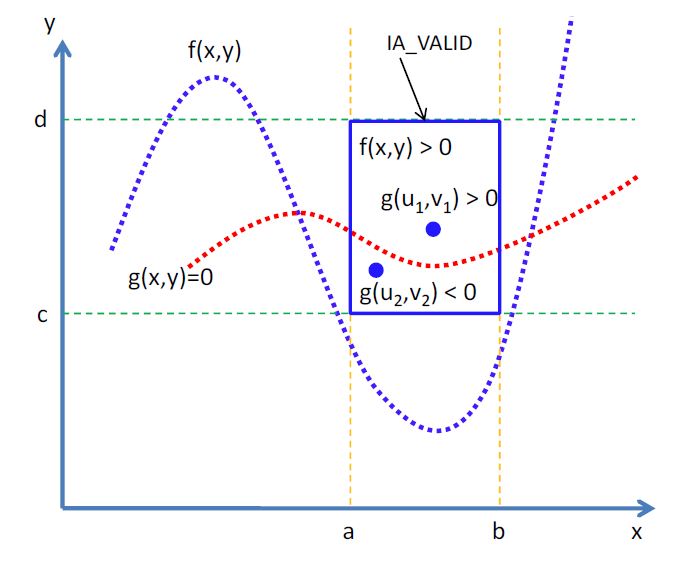
\includegraphics[scale=0.5]{singleEquation.png} 
\caption{Example on solving single equation using the Intermediate Value Theorem} 
\label{fig:single-equation} 
%\end{minipage}
\end{figure} 
{\bf raSAT} first tries to find a box of variables' intervals (by refinements) such that $\bigwedge \limits_{j}^m f_j > 0$ is VALID inside that box. Then it tries to find 2 instances for $g > 0$ and $g < 0$ by testing. 
Intermediate Value Theorem guarantees the existence of an SAT instance in between. 
Note that this method does not find an exact SAT instance. 
\subsection*{Multiple Equations}
The idea of using the Intermediate Value Theorem can also be used for solving multiple equations. Consider $n$ equations ($n \ge 1$): $\bigwedge \limits_{i=1}^n g_i = 0$ and an interval constraint ${\bigwedge\limits_{v_i \in V}v_i \in \langle l_i, h_i \rangle}$. If we can find a set ${\{V_1, \cdots, V_n\}}$ that satisfies the following properties, then we can conclude that $\bigwedge \limits_{i=1}^n g_i = 0$ is satisfiable in ${\bigwedge\limits_{v_i \in V}v_i \in \langle l_i, h_i \rangle}$.
\begin{itemize}
\item[$\bullet$] For all $i = 1, \cdots, n$; we have ${V_i \subset var(g_i)}$.
\item[$\bullet$] For all $i \neq j$, we have $V_i \neq V_j$.
\item[$\bullet$] For all $i = 1, \cdots, n$; let $k_i = |V_i|$ and $V_i = \{v_{ij} \; | \; 1 \le j \le k_i \}$. Then, there exist two values ${(v_{i1}, \cdots, v_{ik_I}) = (x_{i1}, \cdots, x_{ik_i})}$ and ${(v_{i1}, \cdots, v_{ik_I}) = (x'_{i1}, \cdots, x'_{ik_i})}$ such that \[g_i(x_{i1}, \cdots, x_{ik_i}, \cdots, v_{ik}, \cdots) * g_i(x'_{i1}, \cdots, x'_{ik_i}, \cdots, v_{ik}, \cdots) < 0\] for all values of $v_{ik}$ in $\langle l_{ik}, h_{ik} \rangle$ where $v_{ik} \in var(g_i) \setminus V_i$. We denote $ivt(g_i, V_i, \Pi)$ to represent that the polynomial $g_i$ enjoy this property with respect to $V_i$ and $\Pi$.
\end{itemize}
By the first two properties, this method restricts that the number of variables must be greater than or equal to the number of equations.

\begin{example}
Consider two equations $g_1(x, y)=0$ and $g_2(x, y) = 0$ (Figure~\ref{fig:multiple-equations}) which satisfy the above restriction on the number of variables, and the variable intervals is $\Pi = x \in \langle c_1, d_1 \rangle \wedge y \in \langle d_2, c_2 \rangle$. Let $V_1 = \{x\}$ and $V_2 = \{y\}$, we have:
\[g_1(c_1, y)*g_1(d_1, y) < 0 \text{ for all } y \in \langle d_2, c_2 \rangle, \text{ and }\]
\[g_2(x, d_2)*g_2(x, c_2) < 0 \text{ for all } x \in \langle c_1, d_1 \rangle\]
Thus we can conclude that $g_1(x,y)=0 \wedge g_2(x,y=0)$ has a solution inside the box represented by $\Pi$.
\end{example}
\begin{figure}[ht]
\centering
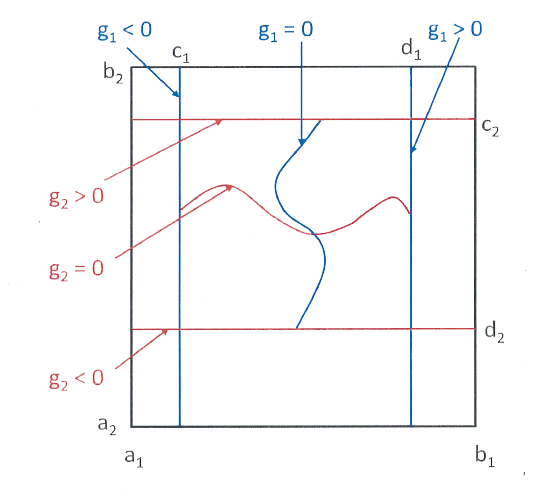
\includegraphics[scale=0.5]{multipleEquations.png} 
\caption{Example on solving single equation using the Intermediate Value Theorem} 
\label{fig:multiple-equations} 
%\end{minipage}
\end{figure}
Our current implementation of handling multiple equations is very naive which is described in Algorithm~\ref{Al:multiple-equations} because for each polynomial, \textbf{raSAT} checks every possible subsets of its variables. As the result, given the constraint $\bigwedge\limits_{i=1}^ng_i=0$, in the worst case \textbf{raSAT} will check $2^{|var(g_1)|}*\cdots*2^{|var(g_n)|}$ cases. As a future work, we may use variables' sensitivity to give priority on subsets of variables.
\begin{algorithm}
\begin{algorithmic}
\Function{equationsProver}{$\bigwedge\limits_{i=j}^ng_i = 0, \Pi, V_0$}
\If {$j > n$} \Comment{All equations are checked}
	\State \Return SAT
\EndIf
\For {$V_j \in P(var(g_j))$} \Comment{$P(var(g_j))$ is the powerset of $var(g_j)$}
	\If {$V_j \cap V = \emptyset$ and $ivt(V', g_j, \Pi)$}
		\State $V_0 \gets V_0 \cup V'$
		\If {\Call{equationsProver}{$\bigwedge\limits_{i=j+1}^ng_i = 0, \Pi, V_0$} = SAT}
			\State \Return SAT
		\EndIf
	\EndIf
\EndFor
\State \Return UNSAT
\EndFunction
\State \Call{equationsProver}{$\bigwedge\limits_{i=1}^ng_i = 0, \Pi, \emptyset$}
\end{algorithmic}
\caption{Solving multiple equations $\bigwedge\limits_{i=1}^n g_i = 0$ with interval constraint ${\Pi = \bigwedge\limits_{v_i \in V} v_i \in \langle l_i, h_i \rangle}$}
\label{Al:multiple-equations}
\end{algorithm}

\subsection*{Experiments on Benchmarks}
In Table \ref{tab:eqexp} we show preliminary experiment for 15 problems that contain polynomial equations in Zankl family. The first 4 columns indicate \emph{name of problems}, \emph{the number of variables}, \emph{the number of polynomial equalities} and \emph{the number of inequalities}  in each problem, respectively. The last 2 columns show comparison results of \textbf{Z3 4.3} and \textbf{raSAT}.
\begin{table}
\centering
\scalebox{1.0}{
\begin{tabular}[b]{|c|c|c|c|c|c|c|c|}
\hline
%\multirow{2}{*}{Problem} & {No.} & {No.} & {No.}&
{Problem} & {No.} & {No.} & {No.}&
\multicolumn{2}{c|}{\textbf{Z3 4.3} (15/15)} &\multicolumn{2}{c|}{\textbf{raSAT} (15/15)}\\
\cline{5-8}
Name & Variables& Equalities& Inequalities&{Result} & {Time(s)}&{Result} & {Time(s)}\\
\hline
gen-03 & 1 & 1 & 0& SAT &0.01 & SAT &0.001\\
\hline
gen-04 & 1 & 1 & 0& SAT &0.01 & SAT &0.001\\
\hline
gen-05 & 2 & 2 & 0& SAT &0.01 & SAT &0.003\\
\hline
gen-06 & 2 & 2 & 1& SAT &0.01 & SAT &0.005\\
\hline
gen-07 & 2 & 2 & 0& SAT &0.01 & SAT &0.002\\
\hline
gen-08 & 2 & 2 & 1& SAT &0.01 & SAT &0.009\\
\hline
gen-09 & 2 & 2 & 1& SAT &0.03 & SAT &0.007\\
\hline
gen-10 & 1 & 1 & 0& SAT &0.02 & SAT &0.002\\
\hline
gen-13 & 1 & 1 & 0& UNSAT &0.05 & UNSAT &0.002\\
\hline
gen-14 & 1 & 1 & 0& UNSAT &0.01 & UNSAT &0.002\\
\hline
gen-15 & 2 & 3 & 0& UNSAT &0.01 & UNSAT &0.03\\
\hline
gen-16 & 2 & 2 & 1& SAT &0.01 & SAT &0.006\\
\hline
gen-17 & 2 & 3 & 0& UNSAT &0.01 & UNSAT &0.03\\
\hline
gen-18 & 2 & 2 & 1& SAT &0.01 & SAT &0.002\\
\hline
gen-19 & 2 & 2 & 1& SAT &0.05 & SAT &0.046\\
\hline
\end{tabular}
}
\caption{Experimental results for 15 equality problems of Zankl family}
\label{tab:eqexp}
\end{table}

\section{Polynomial Constraints over Integers} \label{sec:NIA}

{\bf raSAT} loop can be slightly modified to handle NIA (nonlinear arithmetic over integers) constraints from NRA, 
by setting $\gamma_0 = 1$ in incremental deepening in Section~\ref{sec:incsearch} 
and restricting test data generation on integers. 
We also compare {\bf raSAT} (combination ${(1)-(5)-(8)}$) with {\bf Z3 4.3} on NIA/AProVE benchmark. 
{\bf AProVE} contains 6850 inequalities among 8829. 
Some has several hundred variables, but each API has few variables (mostly just 2 variables). 

The results are, 
\begin{itemize}
\item {\bf raSAT} detects 6764 SAT in 1230.54s, and 0 UNSAT. 
\item {\bf Z3 4.3} detects 6784 SAT in 103.70s, and 36 UNSAT in 36.08s. 
\end{itemize}
where the timeout is $60s$. 
{\bf raSAT} does not successfully solve any unsatisfiable problem, since they have large coefficients
which lead exhaustive search on large area. 
%%%%%%%%%%%%%%%%%
\suppress{
\begin{table*}[t]
\centering
\begin{tabular}{ | l | r | r  r | r | r  | r | r | r | r |}
\hline
    \multicolumn{1}{|l|}{Benchmark} & 
    \multicolumn{5}{c|}{\bf raSAT} & \multicolumn{4}{c|}{\bf Z3 4.3)}\\
\hline
    & \multicolumn{3}{|c|}{SAT} & \multicolumn{2}{|c|}{UNSAT} 
    & \multicolumn{2}{|c|}{SAT} & \multicolumn{2}{|c|}{UNSAT} \\
\hline
AProve (6850) & 6764 & 1230.54 & (s) & 0 & 0.00 & 6784 & 103.70 & 36 & 36.08 
\\
\hline
\end{tabular}
\medskip 
\caption{Comparison on NIA/AProVE} \label{tab:aprove}
\end{table*}
}

%%%%%%%%%%%%%%%%%%%%%%%%%%%%%


\chapter{Related Works} \label{chap:related}
%\section{Methodologies for Polynomial Constraints over Real Numbers}
Although solving polynomial constraints on real numbers is decidable~\cite{tarski}, current methodologies have their own pros and cos. They can be classified into the following categories: 
\begin{enumerate}
\item \textbf{Quantifier Elimination by Cylindrical Algebraic Decomposition (QE-CAD)}~\cite{qecad} 
is a complete technique, and 
is implemented in Mathematica, Maple/SynRac, Reduce/Redlog, QEPCAD-B, and recently 
in
Z3 4.3 (which is referred as nlsat in~\cite{Jovanovic13}).
Although QE-CAD is precise and detects beyond SAT instances (e.g., SAT regions), 
scalability is still challenging, since its complexity is doubly-exponential with respect to the number of variables. 
%Since QE-CAD is DEXPTIME wrt the number of variables, 

\item \textbf{Virtual Substitution } eliminates an existential quantifier by substituting the corresponding quantified variable with a very small value ($-\infty$), and either each root (with respect to that variable) of polynomials appearing in the constraint or each root plus an infinitesimal $\epsilon$. Disjunction of constraints after substitutions is equivalent to the original constraint. Because VS needs the formula for roots of polynomials, its application is restricted to polynomials of degree up to 4. SMT-RAT and  
Z3 \cite{PBM12} applies VS.

\item \textbf{Bit-blasting}. 
In this category of methodology, numerical variables are represented by a sequence of binary variables. The given constraint is converted into another constraint over the boolean variables. SAT solver is then used to find a satisfiable instance of binary variables which can be used to calculate the values of numerical variables.  MiniSmt~\cite{Zankl:2010:SNR:1939141.1939168}, the winner of QF\_NRA in SMT competition 2010, 
applies it for (ir)-rational numbers.
It can show SAT quickly, but due to the bounded bit encoding, 
it cannot conclude UNSAT. In addition, high degree of polynomial results in large SAT formula which is an obstacle of bit-blasting.

\item \textbf{Linearization}. ~
CORD \cite{cordic} uses COrdinate Rotation DIgital Computer (CORDIC) for real numbers to linearizes multiplications into a sequence of linear constraints. Each time one multiplication is linearized, a number of new constraints and new variables are introduced. As a consequence, high degree polynomials in the original constraint lead to large number of linear constraints. 

\item \textbf{Interval Constraint Propagation (ICP)} 
which are used in SMT solver community, e.g., iSAT3~\cite{isat}, 
dReal~\cite{dRealCADE13}, and RSOLVER~\cite{rsolver}. 
ICP combines over-approximation by interval arithmetics and constraint propagation to prune out the set of unsatisfiable points. When pruning does not work, decomposition (branching) on intervals is applied. 
ICP which is capable of solving "multiple thousand arithmetic constraints over some thousands of variables" \cite{isat} is practically often more efficient than algebraic computation.
\end{enumerate}

%Because \textbf{raSAT} in the same category with \text{iSAT3} and \text{dReal}, next section is going to take a look at details of methodologies used in these solvers.
% % % % % % % % % % % % % %

\chapter{Conclusion}


This thesis presented improvement and extensions for an SMT solved {\bf raSAT} including heuristics to deal with exponential exploration of boxes, extensions for handling equations and handling constraints over integer numbers.

\section*{Observation and Discussion} 

From experimental results in Section~\ref{sec:experiments} and~\ref{sec:expsmtlib}, 
we observe the followings. 
\begin{itemize}
\item The degree of polynomials will not affect much. 
\item The number of variables are matters, but also for Z3 4.3. 
The experimental results do not show exponential growth, and we expect 
the strategy of selection of an API in which related intervals are decomposed
seems effective in practice. By observing Zankl examples, we think the maximum 
number of variables of each API seems a dominant factor. 
\item Effects of the number of APIs are not clear at the moment. In simple benchmarks, 
{\bf raSAT} is faster than Z3 4.3, however we admit that we have set small degree $n=6$
for each API. 
\end{itemize}

For instance, {\em matrix-2-all-5,8,11,12} in Zankl 
contain a long monomial (e.g., $60$) with the max degree $6$, and 
relatively many variables (e.g., $14$), which cannot be solved by Z3 4.3, but 
{\bf raSAT} does. 
As a general feeling, if an API contains more than $30 \sim 40$ variables, 
{\bf raSAT} seems saturating. 
We expect that, adding to a strategy to select an API (Section~\ref{sec:intervaldecomp}), 
we need a strategy to select variables in the focus. We expect this can be designed 
with sensitivity (Example~\ref{examp:sensitivity}) and would work in practice. 
Note that sensitivity can be used only with noise symbols in Affine intervals. 
Thus, iSAT and RSOLVER cannot use this strategy, though they are based on IA, too. 

\section*{Future Work}

\medskip \noindent 
{\bf UNSAT core}

\medskip \noindent 
{\bf Exact confirmation}.
Currently, {\bf raSAT} uses iRRAM to verify SAT instances only. 
We are planning to implement confirmation phase to UNSAT cases. 

\medskip \noindent 
{\bf Further strategy refinement}. 
Test data generation, blanced box decomposition


%%%
\suppress{
\subsubsection{Extension of {\bf raSAT} loop}
\begin{itemize}
\item {\bf Equality handling}: currently, {\bf raSAT} loop can handle only inequalities. 
Before applying ideal based technique, such as {\em Gr{\"o}bner basis}, 
we are planning to implement a non-constructive detection of equality 
by {\em intermediate value theorem}. 

\suppress{
\item{\textbf{Polynomial equality by Intermediate value theorem}:} 
Consider 
\begin{center}
$(x_1 \in (a_1,b_1) \wedge \cdots \wedge x_n \in (a_n,b_n))~\bigwedge 
\limits_{j}^m f_j(x_1,\cdots,x_n) > 0~\wedge~g(x_1,\cdots, x_n) = 0.$
\end{center}
SAT can be proved by two steps. First, find a box of the product of 
$(l_{ik},h_{ik}) \subseteq (l_i,h_i)$ (by interval arithmetic) such that 
\begin{center}
$\forall x_1 \in (l_{1k},h_{1k}) \cdots x_n \in (l_{nk},h_{nk}).~\bigwedge 
 \limits_{j}^m f_j(x_1,\cdots,x_n) > 0$~~~~(IA-VALID) 
\end{center}
and find two instances (by testing) in the box with $g(a_1,\cdots,a_n) > 0$ 
and $g(b_1,\cdots,b_n) < 0$. By Intermediate value theorem, we can conclude 
$\exists x_1 \in (l_1,h_1) \cdots x_n \in (l_n,h_n).~g(x_1,\cdots, x_n) = 0$. 
}

\item \textbf{Solving polynomial constraints on integers}: 
In integer domain, the number of test data is finite if interval constraints are bounded. 
Then, Test-UNSAT implies UNSAT if all possible test data are generated. 
A tight interaction between testing and interval decomposition could be investigated.
Mixed integers are also challenging. 
\end{itemize}


\subsubsection{\textbf{raSAT} Development}

\begin{itemize}
\item \textbf{Avoiding local optimal}: 
we borrow an idea of \emph{restart} in MiniSAT for escaping from hopeless local search 
(i.e., solution set is not dense or empty). 
\emph{Heuristics} would be, after a deep interval decomposition of 
a box and Test-UNSAT are reported, backtrack occurs to choose a randomly selected box. 

\item \textbf{Separation of linear constraints}: 
Many benchmarks contain linear constraints. Current implementation does not have 
any tuning, but {\bf raSAT} loop only. 
Practically, separating linear and non-linear constraints and solving them 
in a coordinated way between Presbuger arithmetic and {\bf raSAT} would improve. 
During this separation, variables of intersecting linear constraints would be candidates 
for interval decompositions. 

\item \textbf{Incremental DPLL}: For interactions with the SAT solver, 
we currently apply the very lazy theory learning. Combination with 
\emph{eager} theory propagation would improve, in which we can propagate 
a conflict from a partial truth assignment instead of waiting 
for a full truth assignment obtained by SAT solver.
\end{itemize}
}
%%

%%
\suppress{
\subsection{Applications}
\begin{itemize}
\item \textbf{Checking overflow and roundoff error}: In the computers, the real numbers are represented by finite numbers (i.e., floating point numbers, fixed point numbers). Due to finite representation, the over-flow and roundoff errors (OREs) \cite{ngocsefm, ngocase} may occur. The OREs will be propagated through computations of the program. Further, the computations themselves also cause OREs because the arithmetic needs to round the result to fit the number format. Besides, OREs are also affected by types of statements, i.e., branch, loop, assignment statements.
By symbolic execution, ORE constraints are propagated from a program and ORE problems are reduced to problems of solving ORE constraints for verifying whether OREs occur. 
%For solving ORE constraint, combination of the new form of affine arithmetic ($CAI_1$) and \emph{sensitivity} (i.e., high degrees, )

\item \textbf{Loop invariant generation}: The problem of linear invariant generation is often reduced to the problem of non-linear constraint solving. 
Since Farkas's Lemma \cite{Colon03} uses the product of matrices with polynomial constraint solving, we can extend the target for non-linear invariant generation.
%Based on Farkas' Lemma \cite{Colon03}, non-linear constraints on coefficients of the target linear invariant are generated and a satisfiable instance of these constraints is a candidate of the linear invariant. 
\end{itemize}
}
%%

\bibliographystyle{plainnat}
\bibliography{tungdeptrai}

\end{document}
